\documentclass[xcolor=dvipsnames,leqno]{beamer} 

\usetheme{Copenhagen}
%\beamersetuncovermixins{\opaqueness<1>{25}}{\opaqueness<2->{15}}
\beamertemplatenavigationsymbolsempty

\setbeamertemplate{frametitle}
{
\begin{flushleft}

\color{Blue}
\textbf{\large\insertframetitle}
\end{flushleft}
}

\setbeamertemplate{headline}
{%
  \leavevmode%
  \begin{beamercolorbox}[wd=.5\paperwidth,ht=2ex,dp=1.125ex]{section in head/foot}%
    \hbox to .5\paperwidth{\hfil\insertsectionhead\hfil}
  \end{beamercolorbox}%
  \begin{beamercolorbox}[wd=.5\paperwidth,ht=2ex,dp=1.125ex]{subsection in head/foot}%
    \hbox to .5\paperwidth{\hfil\insertsubsectionhead\hfil}
  \end{beamercolorbox}%
}
\expandafter\def\expandafter\insertshorttitle\expandafter{%
  \insertframenumber\,/\,\inserttotalframenumber} 
\insertsectionhead 
\insertsubsectionhead 

%\usepackage{xcolor}
\usepackage{hyperref}
\usepackage{textcomp}
\usepackage{setspace}
%\usepackage[options]{mcode}
%\usepackage{listings}
\usepackage{algorithmic} 
\usepackage{environ}
\usepackage {mathrsfs}
\NewEnviron{omitframe}{}
\usepackage{lmodern}   
\usepackage{bib entry}
\nobibliography*
\let\newblock\relax
\setbeamertemplate{navigation symbols}{}
\setbeamercolor{upcol}{fg=black,bg=Periwinkle}
\setbeamercolor{lowcol}{fg=black,bg=Periwinkle!40}

\newcommand*{\bigchi}{\mbox{\Large$\chi$}}
\newcommand{\R}{\mathbb{R}}
\renewcommand{\P}{\mathbb{P}}
\newcommand{\E}{\mathbb{E}}
%\newcommand{\C}{\mathbb{C}}
\newcommand{\N}{\mathbb{N}}

\newtheorem{algorithm}{Algorithm}
\newtheorem{thm}{Theorem}
\newtheorem{cor}[theorem]{Corollary}
\newtheorem{lem}[thm]{Lemma}
\newtheorem{prop}{Proposition}
\newtheorem{defn}{Definition}
\newtheorem{rmk}{Remark}
\newtheorem{eg}{Example}   

\title{Stochastic Navier-Stokes Equations perturbed by cylindrical L\'evy noise on 2D rotating sphere}

\author[Leanne Dong]{Leanne Dong\\
\vspace{1cm}{\small Supervised by: Prof. Ben Goldys}}
\vspace{1cm}
\institute[Usyd]{School of Mathematics and Statistics\\
The University of Sydney}
%\titlegraphic{}
\date{November, 2016}
\setbeamersize{text margin left=0.5cm,text margin right=0.5cm}



\begin{document}
%\nobibliography*
	\begin{frame}
	  \titlepage
	\end{frame}

\section[]{Research rationales}  
\begin{frame}{Research rationales}
	\emph{Why study stochastic Navier-Stokes equations {\color{red}with noise, and {\color{red}stable} L\'evy noise}?}
	\begin{itemize}         
		\item More informative than deterministic equations.
		%\item The stochastic Navier-Stokes equations can model turbulence.
		\item To prove in a ``Cheaper" way for unsolved problems.\\
		\begin{itemize}
			\item Clay millenium problem No. 3: Uniqueness in 3D is missing.
			\item At atomic scale, fluid are not continuous fields
	%	\item Model complexity (especially turbulence, whether prediction) requires infinite dimensional analysis.
			\item L\'evy processes are perfect candidates to model discontinuity in infinite dimensions.
		\end{itemize}
	\end{itemize}
	\emph{Why stable-type L\'evy noise ?}
	\begin{itemize}
		\item Has a 'heavy tail' that decays polynomially. Useful for modelling extreme events - earthquakes, stock market crashes.
		\item Allows one to take into account at the same time noise with a large numer of small random impulses and occasionally large random disturbance with infinite moments.
	\end{itemize} 
\end{frame}

\begin{frame}
\frametitle{Research rationales: Rotating spheres?}
\begin{columns}
\column{0.5\textwidth}
\begin{itemize}
	\item Modelling large scale interactions between Ocean and atmosphere requires taking into account that we are on the surface of rotating Earth. 
	\item In cosmology, models of rotating fluids are used to describe many cosmological objects including black holes. (In this case, relativistic effects have to be taken into account which are not included in my thesis)
\end{itemize}
\column{0.5\textwidth}
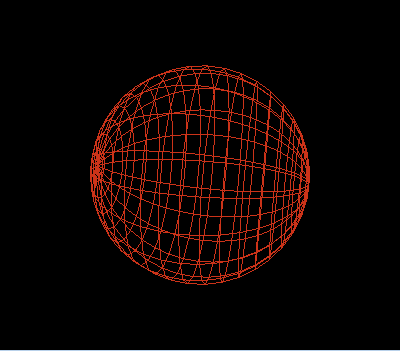
\includegraphics[scale=0.5]{Moving-Sphere.png}
\end{columns}
\end{frame}


\section{Problem formulation}
\begin{frame}[shrink]{The Navier-Stokes equations}
 We consider the stochastic Navier-stokes equations on the 2D unit sphere $\mathbb{S}^2\in (\theta,\phi)$ with rotation. Which is a system of 3 equations:
%\left\{
	\begin{align*}(1)
		\begin{cases}
			\partial_t u+ (u\cdot\nabla)u-\nu L u+\omega\times u+\nabla p=f+\eta(x,t) ,\quad\text{on} \,\, (t, x)\in (0, T)\times\mathbb{S}^2\\
			&\\
			\nabla\cdot u=0,\qquad\text{on} \quad (t, x)\in[0, T)\times\mathbb{S}^2, \quad{\color{RedOrange}\text{Incompressible condition}}\\
			&\\
			u(0)=u_0, \qquad\text{Initial conditions}	
		\end{cases}	
	\end{align*}  
%\right\}	        
\begin{itemize}
	\item $u, p, \nu, f$ are respectively velocity, pressure , viscosity and external forcing.
	\item $L=\Delta + 2\text{Ric}$ is the stress tensor, where $\Delta$ is the Laplace-de Rham operator and $\text{Ric}$ is the Ricci tensor on spheres.
	\item $\omega$ is the Coriolis acceleration which can be formally represented as $\omega(\cdot) = 2\Omega\cos\theta(\cdot)$.
	\item The noise process $\eta(x,t)$ can be viewed as some generalised derivative of $H$-valued L\'evy process.
\end{itemize}
\end{frame}

\begin{frame}
	The sphere can be viewed as a surface embedded into $\R^3$, hence, given any two vector fields $u$, $v$ on $\mathbb{S}^2$, we can find vector fields $\tilde{u}$ and $\tilde{v}$ defined on some nbhd of the surface $\mathbb{S}^2$ such that their restriction to $\mathbb{S}^2$ are equal to, resp. $u$ and $v$, namely,
	\begin{align*}
		\tilde{u}|_{\mathbb{S}^2}=u\in T\mathbb{S}^2\quad\text{and}\quad\tilde{v}|_{\mathbb{S}^2}=v\in T\mathbb{S}^2 
	\end{align*}
So, define orthogonal projection $\pi_x:\R^3\to T_x \mathbb{S}^2$

Then usual spherical calculus can be used to calculate standard curl and div operators.
\end{frame}

\begin{frame}{Weak formulation of Stochastic Navier Stokes Equations}
\begin{itemize}
	\item Orthogonal-projection $P_{\mathcal{L}} : H\to H_{\mathcal{L}}$
	%\item Let $\mathcal{P}$ be the Leray-Hopf operator. It is often written as
	 %it is a matrix valued Fourier multiplier given by
	\begin{align*}
		P_{\mathcal{L}}&=\text{Id}-\Delta^{-1}(\nabla\otimes\nabla).
	\end{align*}
	%It is an orthogonal projection of $(L^2(\mathscr{O}))^2$ onto $E$, which  
 $P_{\mathcal{L}}$	decomposes the velocity vector into its {\color{purple}divergence free part} and the {\color{orange}gradient of the scalar part}, that is, 
	\begin{align*}
		u={\color{purple}P_{\mathcal{L}}[(u\cdot\nabla)u]}+{\color{orange}\nabla \phi}
	\end{align*}
	\item Define $A: D(A)\to H$ by $Au=-\nu P_{\mathcal{L}} L u$, $D(A)=(H^2(\mathbb{S}^2))^2\cap V$.
	\item Define $B: V\times V\to V^{*}$ by $B(u,v)=P_{\mathcal{L}}[(u\cdot\nabla)v]$.
	\item $L(t)=P_{{\mathcal{L}}}\tilde{L}(t)$.%, $\tilde{L}(t)$ is a cylindrical L\'evy process takes value in $E$.    
	\item $B(u)=P_{\mathcal{L}}[\, \text{div}(u\otimes u)\, ]=P_{\mathcal{L}}[\text{div} \, uu^{T}]=B(u,u)$%\mathcal{P}[(u\cdot\nabla) u]$
\end{itemize}	
\end{frame}
\begin{frame}
Then, projecting (1) onto $H$ yields 
\begin{align*}
	\begin{cases}
	u_t=-\nu Au-B(v+z,v+z)-Cv+\alpha z+f,\,\,(t, x)\in (0, T)\times\mathbb{S}^2 \\
		u(0)=u_0\in H
	\end{cases}
\end{align*}
%leads to the abstract equations, which is the version of two-dimensional Stochastic Navier-Stokes equations in $u=u(t)=u(t,x)$ 
Suppose we have solved the projection problem (2) by finding the mild solution $u=P_{\mathcal{L}} u$, how do we recover the pressure from its projection?\\
\vspace{1cm}
\textbf{Answer}: By Hodge decomposition, the pressure satisfies

\[
	\nabla p=\nu\Delta u+(u\cdot\nabla)u-\partial_t \tilde{L}(t)-\mathcal{P}[-\nu\Delta u+(u\cdot\nabla)u-\partial_t \tilde{L}(t)]
\]
Solve for $u$, Substitute $u$ back to (1), we can recover $\nabla p$ in term of forcing term and the solution $u$.
\end{frame}
     
\begin{frame}{My problem}  
Projecting (1) onto $H$ leads to the abstract evolutionary equation in $u=u(t)=u(t,x)$:
	\begin{align*}\tag{2}%\label{iacp1e}
			\begin{cases}
		        du(t)+(Au(t)+B(u(t)))dt+Cu=fdt+GdL(t), \qquad t>0\\
				u(0)=u_0\in V%\,\,x\in\mathbb{R}
			\end{cases}
	\end{align*}  
%Here $G: H\to H$ is a bounded linear operator determines the spatial smoothness of the noise, and $L(t)$ is a $H$-valued L\'evy process.
%The stokes operator $A$ generate a strongly continuous semigroup $\{S(t): t\geq 0\}$ on $H$.

A \textbf{solution} to (2) is a process $\{u(t)\in X,t\geq 0\}$ which can be represented in the form $u(t) = v(t) +z_{\alpha}(t)$, where $\{z_{\alpha}(t), t\in\R\}$ is a stationary Ornstein-Uhlenbeck process $z_{\alpha}$ with drift $-\nu A-C-\alpha I$
	
and $v(t)$ is the solution to the problem (with $v_0 = u_0-z_{\alpha}$):
	\begin{align*}\tag{3}
		\begin{cases}
			\partial_t v = -\nu Av- B(v+z_{\alpha},v+z_{\alpha}) - Cv +\alpha z_{\alpha} +f \\
			v(0)=v_0
		\end{cases}
	\end{align*}
This transformed system is interpreted as an integral equation
\begin{align*}\tag{4}
	v(t)&=S(t)v_0+{\color{orange}\int_{0}^{t}S(t-s)B(v(s)+z_{\alpha}(s)+\alpha z_{\alpha}(s))ds}
\end{align*}
   
\end{frame} 
\begin{frame}{Weak formulation of Stochastic Navier Stokes Equations}
To study the initial value proble (2), one needs to carefully study the properties of stochastic convolution $$z_{\alpha}(t)=\int^t_0 e^{-\hat{A}(t-s)} GdL(s)$$ which satisfies
	\begin{align*}\tag{3}
		\begin{cases}
			dz_{\alpha}(t)+(\nu A + C+\alpha)z_{\alpha}(t)=GdL(t), t\geq 0\\
			z(0)=0
		\end{cases}
	\end{align*}
\end{frame}              

\begin{frame}{Research questions}
	\begin{itemize}
		\item Well-posedness
		\begin{itemize}
			\item Existence, uniqueness of \textbf{weak} and continuous dependence of initial data, forcing and driving noise.
			\item Existence and Uniqueness of a \textbf{strong} solution.
		\end{itemize}
		\item Invariant measures (Existence)
		\item Random Dynamical System: Existence of random attractors
	\end{itemize}
\end{frame}

\subsection{Problem 1: Existence and Uniqueness of solutions $u$}

\begin{frame}{Concepts of solutions: Weak solutions}
	\begin{defn}
	Suppose that $z\in L^4_{\text{loc}}([0,T);\mathbb{L}^4(\mathbb{S}^2)\cap H)$, $ v_0\in H$, $f\in V'$. A weak solution to (2) is a function $v\in C([0,T);H)\cap L^2_{\text{loc}}([0,T);V)$ which satisfies (3) in a weak sense for any $\phi\in V$, $T>0$, and
	\begin{align*}
\partial_t( v,\phi)=( v_0,\phi)-\nu( v,A\phi)-b( v+ z, v+ z,\phi)-( \mathbf{C} v,\phi)+(\alpha z+ f,\phi).
	\end{align*}
Equivalently, (3) holds as an equality in $V'$ for a.e. $t\in[0,T]$. 
\end{defn}
Now if $ f\in H$, and the following regularity is satisfied,
\begin{align*}
	 v\in L^{\infty}(0,T;V)\cap L^2(0,T;D(A)),
\end{align*}
then the solution becomes strong. More precisely,
\end{frame}

\begin{frame}{Concepts of solutions: Strong solutions}
\begin{defn}[Strong solution]\label{ssoln}
Suppose that $z\in L^4_{\text{loc}}([0,T);\mathbb{L}^4(\mathbb{S}^2)\cap H)$, $ v_0\in V$, $f\in H$. We say that $u$ is a \emph{strong solution} of the stochastic Navier-Stokes equations (2) on the time interval $[0,T]$ if $u$ is a weak solution of (2) and in addition
\begin{align*}
	 u\in L^{\infty}(0,T;V)\cap L^2(0,T;D(A)).
\end{align*}
\end{defn}
\end{frame}


\begin{frame}{Problem 1: Well-posedness (Weak sense)}
\textbf{Existence} follows from the Galerkin approximation on spheres. More precisely, this is established in three steps.
	\begin{enumerate}
		\item Construct approximate solutions (Galerkin approximation)

		\item Derive a-priori energy estimates for approximate solutions
			\begin{itemize}
				\item Here I found some uniform apriori estimate on the solution to the transformed equation, and I show that the estimates exist globally in time.
			\end{itemize}
		\item Show approximate solutions converges.
			\begin{itemize}
				\item Extract convergence subsequence, pass to the limit in the equation.
			\end{itemize}
	\end{enumerate}
\textbf{Uniqueness} follows from classical arguments in the spirit of Lion \& Prodi.
\end{frame}  



\begin{frame}{Existence and Uniqueness of weak solutions}
	\begin{thm}
	Assume that $\alpha\ge 0$, $ z\in L^4_{\text{loc}}([0,\infty);\mathbb{L}^4(\mathbb{S}^2)\cap H)$, {\color{red}$ f\in V'$} and $ v_0\in H.$ Then, there exists a unique solution of (4) in the space $D(0,T;H)\cap L^2(0,T;V)$ which belongs to $D(h,T; V)\cap L^2_{\text{loc}}(h,T;D(A))$ for all $h>0$ and $T>0.$ Moreover, if $ v_0\in V$, then $ v\in D(0,T; V)\cap L^2_{\text{loc}}(0,T;D(A))$ for all $T>0.$ In particular, $ v(T,z_n) u^0_n\to  v(T,z_n) u_0$ in $H.$ Moreover, if
	\[\sum_{l=1}^\infty|\sigma_l|^{\beta}\lambda^{\beta/2}_l<\infty\,,\]
	then the theorem holds.
\end{thm}
\end{frame}
\begin{frame}{Existence and Uniqueness of strong solutions}
	\begin{thm}
		Assume that $\alpha\ge 0$, $z\in L^4_{\text{loc}}([0,\infty);\mathbb{L}^4(\mathbb{S}^2)\cap H)$, {\color{red}$ f\in H$} and $ v_0\in H.$ Then, there exists  $\P$-a.s. unique solution of (4) in the space $D(0,T;H)\cap L^2(0,T;V),$ which belongs to $D(\epsilon,T; V)\cap L^2_{\text{loc}}(\epsilon,T;D(A))$ for all $\epsilon>0,$ and $T>0.$ Moreover, if $ v_0\in V$, then $ u\in D(0,T; V)\cap L^2_{\text{loc}}(0,T;D(A))$ for all $T>0$, $\omega\in\Omega$. Moreover, if
	\[\sum_{l=1}^\infty|\sigma_l|^{\beta}\lambda^{\beta/2}_l<\infty\,,\]
	then the theorem holds.
	\end{thm}
\begin{proof}
	We follow a classical fixed point typed argument of Lion\& Prodi, also in \cite{MR1207308}. This consists of proving {\color{red}Local existence and uniqueness} and {\color{red}Uniform apriori estimates}.
\end{proof}
\end{frame}
 

\subsection{Problem 2: Existence of invariant measures}

\begin{frame}{What is invariant measures?}
	Roughly speaking, it is a stationary solution represents the long time behaviour of a given dynamical system. 

\begin{align*}
\textbf{Markov semigroup}\qquad (P_t\phi)(u_0) = \E_{u_0}\phi(u_t)
\end{align*}

\begin{align*}
\textbf{Invariant measure}\qquad	\int P_t(u_0, A)d\mu(u_0)&=\mu(A)\\ 
P^*_t\mu &= \mu 
\end{align*}

\begin{align*}
\textbf{Birkoff Ergodic Theorem}\qquad	\frac{1}{T}\int^T_0\phi(u_t)\,dt =\int \phi(u)\,d\mu(u)
\end{align*}
\end{frame}

\begin{frame}{How to prove invariant measures?}
	\begin{enumerate}
		\item It is worth mentioning that the existence of invariant measures was not possible for the deterministic Navier-Stokes Equations. This motivates us to study the same question in ``stochastic'' sense.
		\item  In standard case of equations with \textbf{Gaussian} noise, existence of invariant measures can be established via three criterions.
		\begin{itemize}
			\item Markov property
			\item Feller property
			\item Tightness of probability law
		\end{itemize}
		The first two properties follow from well-posedness. Tightness follows from Krylov-Bogoliubov argument for Markov process.
	\end{enumerate}
Fir the SNSE with stable typed noise, existence of invariant measures is a more difficult problem compared to the Gaussian counterpart. This is because the energy estimates for 2nd moments of the solution are not available, which fails the standard argument (SLLN)
\end{frame}

\subsection{Problem 3: Existence of random attractors}

\begin{frame}{Random Dynamical Systems: preliminary}
	\begin{defn}\label{defnrds}
    Given a metric DS $\mathfrak{T}$ and a Polish space $(X,d)$, a map $\varphi:\R\times\Omega\times X\ni (t,\omega,x)\mapsto\varphi(t,\omega)x\in X$ is called a \emph{measurable random dynamical system} (on $X$ over $\vartheta$), iff
\begin{itemize}
    \item $\varphi$ is $(\mathcal{B}(\R)\times\mathcal{F}\times\mathcal{B},\mathcal{B})$-measurable.
    \item The trajectories $\varphi(\cdot,\omega)x:\R\to X$ are c\`adl\`ag $\forall\,(\omega,x)\in\Omega\times\R$;
    \item $\varphi$ is $\vartheta$-cocycle:
\begin{align*}
    \varphi(t+s,\omega)=\varphi(t,\vartheta_s\omega)\circ\varphi(s,\omega)\quad\forall\quad s,t\in\R,\,\,\varphi(0,\omega)=\text{id},\,\,\forall\,\,\omega\in\Omega.
\end{align*}   
The concept of RDS is a relative new development combining ideas and methods from probability theory and dynamical systems.
\end{itemize}

%A RDS is said to be continuous or differentiable iff. $\forall\,(t,\omega)\in\R\times\Omega$, $\varphi(t,\cdot,\omega): X\to X$ is continuous or differentiable, respectively. Likewise, $\varphi$ is said to be c\`adl\`ag  iff. for all $\omega\in\Omega$ and $x\in X$, the map $\varphi(\cdot,\omega,x):\R\to X$ is c\`adl\`ag.
\end{defn}
\end{frame}

\begin{frame}{Random Dynamical Systems: preliminary}
\begin{enumerate}
	\item  \textbf{Attractor} is a central notion from mathematical physics, which conveys crucial geometric information about the asymptotic regime of a dynamical system as $t\to \infty$.
	\item  Now, given a probability space, a \textbf{Random Attractor} is a compact random set, invariant for the associated RDS and attracting every bounded random set in its basis of attraction.
\end{enumerate}
 More precisely,

\end{frame}

\begin{frame}{Existence of random attractors}
	\begin{defn} A random set $A:\Omega\to\mathfrak{C} (X)$ is a \emph{random attractor} iff
\begin{itemize}
    \item $A$ is a compact random set;
    \item $A$ is $\varphi$-invariant, i.e. $\P$-a.s.
    \begin{align}
        \varphi(t,\omega)A(\omega)=A(\vartheta_t\omega),
    \end{align}
    \item $A$ is attracting, in the sense that, for all $B\in X$ it holds
\begin{align*}
    \lim_{t\to\infty}\rho(\varphi(t,\vartheta_{-t}\omega)B(\varphi_{-t}\omega),A(\omega))=0.
\end{align*}
\end{itemize}
\end{defn}
\end{frame}

\begin{frame}{Existence of random attractors: Proof}
	I proved the existence of random attractor using a simple argument inspired from Flandoli and Crauel \cite{MR1305587}. Namely in three steps,
\begin{enumerate}
	\item Using an apriori estimate for the strong solution. (i.e. a strong solution bounded in $V$ and compact in $H$)
	\item Using these estimates, we prove, respectively the existence of an absorbing ball in $H$ at $t=-1$ and $V$ at $t=0$.
	\item Using compact embedding of Sobolev spaces, we identified a compact absorbing set and consequently deduce the existence of a random attractor.
\end{enumerate}
\end{frame}
\subsection{Auxiliary results in stochastic analysis}
\begin{frame}{Fubini theorem for stochastic integral w.r.t. large and small jumps}
	We proved a new version of stochastic Fubini Theorem for the subordinated process $L(t)=W(Z(t))$, where $W$ is a cylindrical Wiener process on Hilbert space and $Z$ is a subordinator process. Our stochastic Fubini theorem capture both large and small jumps that states the following.
\begin{thm}\label{sfubini}
\begin{align*}\tag{5}
	\int_0^T\left(\int_0^s \Phi(s,\sigma)dL(\sigma)\right)ds=\int_0^T\left(\int_{\sigma}^T \Phi(s,\sigma)ds\right)dL(\sigma).
\end{align*}
\end{thm}
Some technical conditions required are 
\end{frame}

\begin{frame}
\begin{enumerate}
	\item $U$  and $E$ be separable Hilbert spaces.
	\item $(\Omega,\mathcal{F},\P)$ is a probability space, $T>0$ is fixed
	\item The mapping $[0,T]\times[0,T]\times\Omega\ni (s,\sigma,\omega)\mapsto \Phi(s,\sigma,\omega)\in L(U,E)$ is a strongly measurable with respect to the $\sigma$-algebra $\mathcal B([0,T])\otimes\mathcal P_T$, where $\mathcal P_T$ stands for the predictable $\sigma$-algebra in $[0,T]\times\Omega$. More precisely, we assume that for every $y\in U$ the mapping $[0,T]\times[0,T]\times\Omega\ni (s,\sigma,\omega)\mapsto \Phi(s,\sigma,\omega)y\in E$ is measurable with respect to the $\sigma$-algebra $\mathcal B([0,T])\otimes\mathcal P_T$. 
	\item Furthermore, assume that $L$ is a $U$-valued L\'evy process defined as $L(t):=W(Z(t))$, $Z(t)$ is a subordinator process belonging to Sub($p$), i.e. $Z(t)$ has intensity measure satisfying
	\begin{align*}
	\rho(\{0\})=0,\quad\int_1^{\infty}\rho(d\xi)+\int_0^1\xi\rho(d\xi)<\infty\quad	\int_0^1\xi^{\frac{p}{2}}\rho(d\xi)<\infty,
	\end{align*}
	where $\rho$ and $\nu$ are respectively the intensity measure on $\R$ and L\'evy measure on $U_0$. One relates $\rho$ and $\nu$ as
	\begin{align*}
	\nu(\Gamma)=\int_0^{\infty}\zeta_s(\Gamma)\rho(ds),\quad\Gamma\in\mathcal{B}(Y).
	\end{align*}
\end{enumerate}

\end{frame}
\section{References}

\begin{thebibliography}{9}
\bibitem{MR1305587} 
Hans Crauel and Franco Flandoli.
\textit{Attractors for random dynamical systems}. 
Probab. Theory Related Fields, 100(3), 1994


\bibitem{MR1207308} 
Zdzislaw, Brzezniak, Marek Capinski and Franco Flandoli.
\textit{Pathwise global attractors for stationary random dynamical systems}. 
Probab. Theory Related Fields, 95(1), 1993

\end{thebibliography}

\begin{center}
\Huge {\color{Plum}Thank You!}
\end{center}

\end{document}